%\usebackgroundtemplate{%             declare it
%	\tikz[overlay,remember picture] \node[opacity=1, at=(current page.center)] {
%		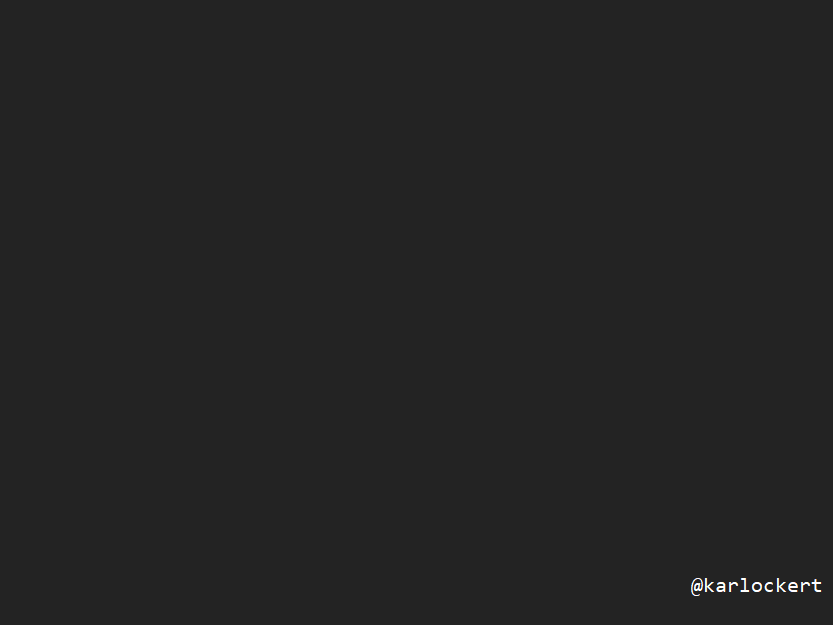
\includegraphics[height=\paperheight]{img/bakgrunn.png}};}

\begin{frame}[noframenumbering, plain]
%	\FrameText{@\href{https://www.twitter.com/Karlockert}{karlockert}}
	%	\frametitle{Hvis du ønsker}
	
		\begin{block}{\color{white}\textbf{\Large{The Hubbard Model }}}
			\vspace{-10pt}\rule{\textwidth}{0.5pt}
			\color{white}
			The Hubbard model is often called the ``Ising model'' of strongly correlated quantum systems, and an exact solution to this lattice model is only known in one dimension except in special limits.  
			It is given by the Hamiltonian 
		\end{block}
		{\large
			
%			\begin{tcolorbox}
				\begin{equation*}
					\mathcal{H} = - \sum_{i,j,\sigma}t_{ij}c_{i\sigma}^{\dagger}c_{j\sigma} + \sum_{i,\sigma}U_i n_{i,\sigma}n_{i,-\sigma}.
				\end{equation*}
%			\end{tcolorbox}
		}
	\begin{block}{}\color{white}
	where the first term is a tight-binding approximation of the system near its Fermi-energy, and the second term describes the on-site energy cost of having doubly occupied lattice sites. 
\end{block}
	%	hvor $O$ er en operator som korresponderer til en observerbar størrelse og $\mathcal{H}$ er Hamiltonian til systemet.
\end{frame}